\chapter[Análisis Dimensional]{Análisis Dimensional y Teoria de Modelos}

	
	En experimentos normalmente el número de variables que intervienen
	es muy grande. El análisis dimensional permite reducir el número de
	variables mediante el cálculo de \textcolor{red}{grupos adimensionales}.
	
	El análisis de los datos experimentales es así mucho más claro y sencillo.
	
	El ejemplo más típico es el de arrastre de un flujo sobre una esfera.
	Si diseñamos un experimento para estudiar éste arrastre en funcón
	de las variables físicas, debemos tener en cuenta las variaciones
	de 
	\begin{itemize}
		\item {el diámetro de la esfera, $d$} 
		\item {la velocidad del flujo, $v$} 
		\item {la densidad del fluido, $\rho$} 
		\item {la viscosidad del fluido, $\mu$} 
	\end{itemize}
	Ésto representan muchos experimentos.

	
	Sin embargo, el Análisis Dimensional permite demostrar que sólo hay
	que considerar dos variable o grupos adimensionales. Es usual usar
	los grupos 
	\[
	\frac{F_{D}}{\frac{1}{2}\rho v^{2}S}
	\]
	y 
	\[
	\frac{\rho vd}{\mu}
	\]
	
	Esto nos permite hacer experimentos variando únicamente la velocidad
	$v$, sin preocuparnos por la densidad, diámetro, viscosidad, \ldots{}
	Dos experimentos con la misma relación $\frac{\rho vd}{\mu}$ nos
	darán como resultado la misma relación $\frac{F_{D}}{\frac{1}{2}\rho v^{2}S}$.
	
	Ésto es útil para experimentar sobre modelos a escala de un diseño,
	sin fabricar el prototipo, que puede ser caro. El modelo ha de ser
	\textcolor{green}{geométricamente similar} al prototipo. Si la relación
	$\frac{\rho vd}{\mu}$ es también igual se dicen que el modelo y el
	prototipo son \textcolor{green}{dinámicamente similares}.

	
	\subsection*{Ejemplo:}
		Se mide la fuerza de arrastre que actúa sobre una esfera de  de diámetro
		en agua a  con una velocidad de  y se observa que es . ?`Cuál debería
		ser la velocidad para una esfera de  de diámetro en aire estándar
		a nivel del mar para qe los experimentos sean dinámicamente similares?
		?`Y cuál sería la fuerza medida?
		
		La densidad del agua es $\rho_{1}=1000\,\text{Kg}/\text{m}^{3}$,
		y la viscosidad es $\mu_{1}=10^{-3}\,\text{Pa}\cdot\text{s}$, de
		forma que 
		\[
		\frac{\rho_{1}v_{1}d_{1}}{\mu_{1}}=\frac{(1000\,\text{Kg}/\text{m}^{3})(2\,\text{m/s})(0.08\,\text{m})}{10^{-3}\,\text{Pa}\cdot\text{s}}=1.6\times10^{5}
		\]
		y 
		\[
		\frac{{F_{D}}_{1}}{\frac{1}{2}\rho_{1}v_{1}^{2}S_{1}}=\frac{5\,\text{N}}{0.5(1000\,\text{Kg}/\text{m}^{3})(2\,\text{m/s})^{2}\pi(0.04\,\text{m})^{2}}=0.497
		\]

		La densidad y la viscosidad del aire a $20\,^{\circ}C$ son, respectivamente,
		$\rho_{2}=1.2\,\text{Kg}/\text{m}^{3}$ y $\mu_{2}=1.8\times10^{-5}\,\text{Pa}\cdot\text{s}$,
		de forma que, si han de ser dinámicamente similares, 
		\[
		\frac{\rho_{2}v_{2}d_{2}}{\mu_{2}}=\frac{(1.2\,\text{Kg}/\text{m}^{3})v_{2}(1.5\,\text{m})}{1.8\times10^{-5}\,\text{Pa}\cdot\text{s}}=1.6\times10^{5}
		\]
		
		\[
		\Rightarrow v_{2}=1.6\,\text{m/s}
		\]
		y la fuerza medida será 
		\[
		\frac{{F_{D}}_{2}}{\frac{1}{2}\rho_{2}v_{2}^{2}S_{2}}=\frac{{F_{D}}_{2}}{0.5(1.2\,\text{Kg}/\text{m}^{3})(1.6\,\text{m/s})^{2}\pi(0.75\,\text{m})^{2}}=0.497
		\]
		
		\[
		\Rightarrow{F_{D}}_{2}=1.35\,\text{N}
		\]
	

\section{El Teorema $\Pi$ de Buckingham}

	
	Los productos adimensionales de variables físicas, como $\frac{F_{D}}{\frac{1}{2}\rho v^{2}S}$
	y $\frac{\rho vd}{\mu}$ reciben el nombre de \textcolor{green}{grupos
		adimensionales}, o \textcolor{green}{grupos $\Pi$}. Muchas veces
	reciben nombre propios. A $\frac{F_{D}}{\frac{1}{2}\rho v^{2}S}$
	se le denota como $C_{D}$, y es el coeficiente de arrastre. $\frac{\rho vd}{\mu}$
	es $\text{Re}$, el número de Reynolds.
	
	Veamos cómo se calculan de forma general estos grupos:
	
	La variables físicas vienen definidas en un conjunto de dimensiones
	básicas. Estas dimensiones suelen ser la masa ($M$), la longitud
	($L$) y el tiempo($T$). 
	
	{\footnotesize{}En problemas con variables termodinámicas podemos
		también tener la temperatura ($\Theta$), pero en general el número
		de dimensiones básicas será 3.}{\footnotesize\par}
	
	En las siguientes tablas se listan algunas variables físicas importantes,
	sus dimensiones y sus unidades en S.I.

	\bigskip

\renewcommand{\arraystretch}{1.3} % Para cambiar altura de filas en la tabla
\begin{tabular}{|c|c|c|c|}
	\hline 
	\textbf{Magnitud}  & \textbf{Símbolo}  & \textbf{Dimensiones}  & \textbf{Sistema Internacional} \tabularnewline
	\hline 
	\hline 
	longitud  & $l$  & $\text{L}$  & $\text{m}$ \tabularnewline
	\hline 
	tiempo  & $t$  & $\text{T}$  & $\text{s}$ \tabularnewline
	\hline 
	masa  & $m$  & $\text{M}$  & $\text{Kg}$ \tabularnewline
	\hline 
	fuerza  & $F$  & $\text{M}\,\text{L}\,\text{T}^{-2}$  & N \tabularnewline
	\hline 
	velocidad  & $v$  & $\text{L}\,\text{T}^{-1}$  & $\text{m}/\text{s}$ \tabularnewline
	\hline 
	aceleración  & $a$  & $\text{L}\,\text{T}^{-2}$  & $\text{m}/\text{s}^{2}$ \tabularnewline
	\hline 
	energía  & $E$  & $\text{M}\,\text{L}^{2}\,\text{T}^{-2}$  & $\text{J}$ \tabularnewline
	\hline 
	potencia  & $P$ (o $N$)  & $\text{M}\,\text{L}^{2}\,\text{T}^{-3}$  & $\text{W}$ \tabularnewline
	\hline 
	área  & $A$ (o $S$)  & $\text{L}^{2}$  & $\text{m}^{2}$\tabularnewline
	\hline 
	volumen  & $V$  & $\text{L}^{3}$  & $\text{m}^{3}$ \tabularnewline
	\hline 
	caudal  & $Q$  & $\text{L}^{3}\,\text{T}^{-1}$  & $\text{m}^{3}/\text{s}$ \tabularnewline
	\hline 
	flujo másico  & $\dot{m}$  & $\text{M}\,\text{T}^{-1}$  & $\text{Kg}/\text{s}$ \tabularnewline
	\hline 
	presión  & $p$  & $\text{M}\,\text{L}^{-1}\,\text{T}^{-2}$  & $\text{Pa}$ \tabularnewline
	\hline 
	gravedad  & $g$  & $\text{L}\,\text{T}^{-2}$  & $\text{m}/\text{s}^{2}$ \tabularnewline
	\hline 
	densidad  & $\rho$  & $\text{M}\,\text{L}^{-3}$  & $\text{Kg}/\text{m}^{3}$ \tabularnewline
	\hline 
	peso específico  & $\gamma$  & $\text{M}\,\text{L}^{-2}\,\text{T}^{-2}$  & $\text{N}/\text{m}^{3}$ \tabularnewline
	\hline 
	viscosidad dinámica  & $\mu$  & $\text{M}\,\text{L}^{-1}\,\text{T}^{-1}$  & $\text{Kg}/\text{m}\,\text{s}$ (o $\text{Pa}\,\text{s}$) \tabularnewline
	\hline 
	viscosidad cinemática  & $\nu$  & $\text{L}^{2}\,\text{T}^{-1}$  & $\text{m}^{2}/\text{s}$ \tabularnewline
	\hline 
	velocidad del sonido  & $c$  & $\text{L}\,\text{T}^{-1}$  & $\text{m}/\text{s}$ \tabularnewline
	\hline 
	tensión superficial  & $\sigma$  & $\text{M}\,\text{T}^{-2}$  & $\text{N}/\text{m}$ \tabularnewline
	\hline 
	módulo de compresibilidad  & $B$  & $\text{M}\,\text{L}^{-1}\,\text{T}^{-2}$  & $\text{Pa}$ \tabularnewline
	\hline 
	temperatura  & $T$  & $\Theta$  & K\tabularnewline
	\hline 
	conductividad térmica  & $k$  & $\text{M}\,\text{L}\,\text{T}^{-3}\,\Theta^{-1}$  & $\text{W}/\text{m}\,\text{K}$ \tabularnewline
	\hline 
	difusividad térmica  & $\alpha$  & $\text{L}^{2}\,\text{T}^{-1}$  & $\text{m}^{2}/\text{s}$ \tabularnewline
	\hline 
	difusividad  & $\mathcal{D}$  & $\text{L}^{2}\,\text{T}^{-1}$  & $\text{m}^{2}/\text{s}$ \tabularnewline
	\hline 
	capacidad calorífica  & $c_{p}$  & $\text{L}^{2}\,\text{T}^{-2}\,\Theta^{-1}$  & $\text{J}/\text{Kg}\,\text{K}$ \tabularnewline
	\hline 
\end{tabular}
\renewcommand{\arraystretch}{1}
	\bigskip

	El Teorema $\Pi$ de Buckingham garantiza que, \textcolor{blue}{dado
		un cierto fenómeno descrito por $n$ variables f\'{i}sicas, éste
		número puede reducirse a una relación de $k$ grupos adimensionales,
		donde $j=n-k$ es igual al número de variables que no pueden formar
		un $\Pi$ y siempre es igual o menor que el número de dimensiones
		que describen las variables.}
	
	Para formar los $\Pi$'s, seleccionamos $j$ variables independientes
	(en el sentido de que no pueden formar ellas solas un $\Pi$), y escribimos
	cada grupo adimensional añadiendo al producto general de potencias
	de estas variables cada una del resto de las variables, que puede
	estar elevada a una cierta potencia también. Cada una de estas combinaciones
	ha de ser adimensional. De esta condición se obtienen las potencias
	adecuadas de las variables.
	
	Parece un poco complicado, pero en realidad es muy simple y tan sólo
	hace falta un poco de práctica. Veamos un ejemplo.

	
	\subsection*{Ejemplo:}
		En el arrastre de la bola, sabemos que intervienen:
		
		- la fuerza de arrastre $F_{D}$, que es la variable dependiente,
		y que tiene unidades $N$, es decir, $MLT^{-2}$ 
		
		- el diámetro de la bola, $d$, con unidades $L$ 
		
		- la velocidad del flujo $v$, con $LT^{-1}$ 
		
		- la densidad del fluido $\rho$, con $ML^{-3}$ 
		
		- la viscosidad del fluido $\mu$, con $ML^{-1}T^{-1}$ 
		
		$j$ será como mucho 3, debido a que no tenemos la temperatura $\Theta$.
		Después de estudiar el sistema, vemos que $\rho$, $v$ y $d$ ser\'{i}a
		una buena selección, ya que no pueden formar un $\Pi$, y son bastante
		generales. Evidentemente, hay múltiples posibilidades correctas. Habrán
		entonces $5-3=2$ grupos adimensionales.
		
		El primer $\Pi$ lo fomariamos como 
		\[
		\Pi_{1}=\rho^{a}v^{b}d^{c}F_{D}
		\]
		
		Como ha de ser adimensional, las potencias $a$, $b$ y $c$ han
		de ser tales que se anulen las potencias de cada dimensión, es decir,
		\[
		(ML^{-3})^{a}(LT^{-1})^{b}(L)^{c}(MLT^{-2})=M^{0}L^{0}T^{0},
		\]
		y de aquí obtenemos tres ecuaciones para las potencias, 
		\begin{eqnarray*}
			\begin{cases}
				a+1 & =0\\
				-3a+b+c+1 & =0\\
				-b-2 & =0
			\end{cases}
		\end{eqnarray*}
		cuya solución es $(a=-1,b=-2,c=-2).$
		
		Por tanto, 
		\[
		\Pi_{1}=\rho^{-1}v^{-2}d^{-2}F_{D}=\frac{F_{D}}{\rho v^{2}d^{2}}.
		\]
		El coeficiente de arrastre $C_{D}$ es proporcional a este $\Pi$.

		El segundo $\Pi$ lo calculamos añadiendo la viscosidad al producto
		de las tres potencias de las variables, $\Pi_{2}=\rho^{a}v^{b}d^{c}\mu$,
		y la relación para obtener las potencias será 
		\[
		(ML^{-3})^{a}(LT^{-1})^{b}(L)^{c}(ML^{-1}T^{-1})=M^{0}L^{0}T^{0},
		\]
		que dará lugar al sistema 
		\begin{eqnarray*}
			\begin{cases}
				a+1 & =0\\
				-3a+b+c-1 & =0\\
				-b-1 & =0
			\end{cases}
		\end{eqnarray*}
		cuya solución es $a=b=c=-1.$
		
		Por tanto, 
		\[
		\Pi_{2}=\rho^{-1}v^{-1}d^{-1}\mu=\frac{\mu}{\rho vd}.
		\]
		El número de Reynolds es el inverso de este $\Pi$.

	
	\subsection*{Actividad 1:}
		La potencia consumida por una bomba es función del caudal $Q$, el
		tamaño de la bomba $D$ (es el diámetro externo del rodete, por ejemplo),
		la velocidad angular $\omega$, la densidad del fluido $\rho$ y su
		viscosidad $\mu$. Escribir como relación adimensional.
		
\section{Números adimensionales básicos}
	
	
	Existe una serie de grupos adimensionales clásicos en Mecánica de
	Fluidos. Algunos son más importantes que otros. En total existen cientos,
	pero en la siguiente tabla sólo vamos a indicar los más usados.
	
	
	
\renewcommand{\arraystretch}{1.3}	
	\begin{tabular}{|>{\raggedright}p{0.2\textwidth}|>{\centering}p{0.2\columnwidth}|>{\raggedright}p{0.5\textwidth}|}
		\hline 
		\textcolor{red}{número de Reynolds}{ } & {$\text{Re}=\frac{\rho uL}{\mu}$ } & {El más importante. Interviene siempre o casi siempre }\tabularnewline
		\hline 
		\textcolor{red}{número de Euler}{ } & {$\text{Eu}=\frac{\Delta p}{\rho u^{2}}$ } & {Si $\Delta p$ está relacionada con la presión de vapor, éste
			número es el }\textcolor{red}{coeficiente de cavitación}{ }\tabularnewline
		\hline 
		\textcolor{red}{número de Froude}{ } & {$\text{Fr}=\frac{u^{2}}{gL}$ } & {Flujos con superficie libre }\tabularnewline
		\hline 
		\textcolor{red}{número de Weber}{ } & {$\text{We}=\frac{\rho u^{2}L}{\sigma}$ } & {Flujos con superficie libre. $\sigma$ és la tensión superficial }\tabularnewline
		\hline 
		\textcolor{red}{número de Mach}{ } & {$\text{Ma}=\frac{u}{c}$ } & {Flujos compresibles. $c$ es la velocidad del sonido }\tabularnewline
		\hline 
		\textcolor{red}{número de Rossby}{ } & {$\text{Ro}=\frac{u}{\Omega L}$ } & {Flujos geof\'{i}sicos. $\Omega$ es la velocidad angular
			de la Tierra }\tabularnewline
		\hline 
		\textcolor{red}{coeficiente adiabático}{ } & {$\gamma=\frac{c_{p}}{c_{v}}$ } & { Flujos compresibles }\tabularnewline
		\hline 
		\textcolor{red}{número de Prandtl}{ } & {$\text{Pr}=\frac{\mu c_{p}}{k}$ } & { Convección térmica }\tabularnewline
		\hline 
		\textcolor{red}{número de Ecker}{ } & {$\text{Ec}=\frac{u^{2}}{c_{p}T_{0}}$ } & { Disipación térmica }\tabularnewline
		\hline 
		\textcolor{red}{número de Strouhal}{ } & {$\text{St}=\frac{\omega L}{u}$ } & { Flujos oscilatorios }\tabularnewline
		\hline 
		\textcolor{red}{rugosidad relativa y coeficiente de fricción}{ } & {$\frac{\epsilon}{D},\quad f=\frac{\Delta h_{r}}{\frac{L}{D}\frac{u^{2}}{2g}}$ } & { Flujos en tuber\'{i}as }\tabularnewline
		\hline 
		\textcolor{red}{coeficientes de presión} & {$C_{p}=\frac{p-p_{\infty}}{\frac{1}{2}\rho u^{2}}$ } & {Aerodinámica }\tabularnewline
		\hline 
		\textcolor{red}{coef. de sustentación}{ } & {$C_{L}=\frac{F_{L}}{\frac{1}{2}\rho u^{2}S}$ } & {Aerodinámica }\tabularnewline
		\hline 
		\textcolor{red}{coef. de arrastre}{ } & {$C_{D}=\frac{F_{D}}{\frac{1}{2}\rho u^{2}S}$ } & { Aerodinámica }\tabularnewline
		\hline 
	\end{tabular}
	\renewcommand{\arraystretch}{1}


\section{Adimensionalización de ecuaciones}

	
	
	En muchas ocasiones, es interesante escribir las ecuaciones básicas
	en forma adimensional. De esta forma se estan describiendo fenómenos
	con independencia de la magnitud de las escalas, y se puede apreciar
	mejor la relación entre términos.
	\subsection*{Ejemplo:}
		Como ejemplo, vamos a adimensionalizar la ecuación de Navier-Stokes
		para flujo incompresible (ver sesión ''Conservación de cantidad de
		movimiento II'') para el estudio típico de una esfera de diámetro
		$D$ en una corriente de un flujo con velocidad $V$ de un fluido
		de densidad $\rho$ y viscosidad $\mu$,
		\[
		\dparc{\vec{u}}{t}+\left(\vec{u}\cdot\vec{\nabla}\right)\vec{u}=\vec{g}-\frac{1}{\rho}\vec{\nabla}p+\frac{\mu}{\rho}\triangle\vec{u}
		\]
		

			En el problema que se está estudiando tenemos una velocidad de referencia
			$U$ y una longitud de referencia $D$. La velocidad y la posición
			pueden ser escritas de forma adimensional tomando estas magnitudes
			como referencia 
			\[
			\vec{u}^{\ast}=\frac{\vec{u}}{U}\quad;\quad\vec{r}^{\ast}=\frac{\vec{r}}{D}
			\]
			%
\begin{center}
	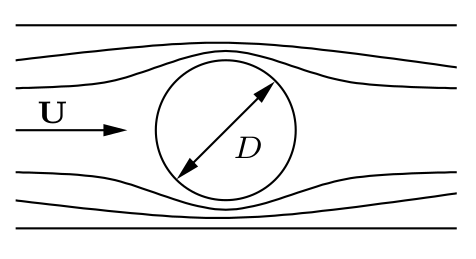
\includegraphics[width=0.5\linewidth]{TeX_files/chapter06-ADimensional/esfera}
\end{center}

		
		No olvidemos que estas relaciones son vectoriales, 
		\[
		\left\{ \begin{array}{l}
			u_{x}^{\ast}=\frac{u_{x}}{U}\\
			u_{y}^{\ast}=\frac{u_{y}}{U}\\
			u_{z}^{\ast}=\frac{u_{z}}{U}
		\end{array}\right.\quad;\quad\left\{ \begin{array}{l}
			x^{\ast}=\frac{x}{D}\\
			y^{\ast}=\frac{y}{D}\\
			z^{\ast}=\frac{z}{D}
		\end{array}\right.
		\]
		
		El tiempo adimensional se puede calcular usando como referencia $D/V$,
		que tiene dimensiones de tiempo, $t^{\ast}=\frac{t}{\frac{D}{U}}=\frac{tU}{D},$ 
		
		la gravedad adimensional es $\vec{g}^{\ast}=\frac{\vec{g}}{\frac{U^{2}}{D}}=\frac{D\vec{g}}{U^{2}},$ 
		
		y la presión adimensional es $p^{\ast}=\frac{p}{\rho U^{2}}.$
		
		Por otro lado, hay que tener en cuenta que las derivadas también son
		adimensionales, 
		\[
		\dparc{}{x}=\dparc{}{\left(Dx^{\ast}\right)}=\frac{1}{D}\dparc{}{x^{\ast}}\,\Rightarrow\,\left\{ \begin{array}{l}
			\vec{\nabla}=\frac{1}{D}\vec{\nabla}^{\ast}\\
			\\
			\triangle=\frac{1}{D^{2}}\triangle^{\ast}
		\end{array}\right.
		\]
		
		Adimensionalización de los términos de la Ecuación de Navier-Stokes:
		\begin{eqnarray*}
			\dparc{\vec{u}}{t} & = & \dparc{\left(U\vec{u}^{\ast}\right)}{\left(\frac{D}{U}t^{\ast}\right)}=\frac{U^{2}}{D}\dparc{\vec{u}^{\ast}}{t^{\ast}}\\
			\left(\vec{u}\cdot\vec{\nabla}\right)\vec{u} & = & \left(\left(U\vec{u}^{\ast}\right)\cdot\frac{1}{D}\vec{\nabla}^{\ast}\right)\left(U\vec{u}^{\ast}\right)=\frac{U^{2}}{D}\left(\vec{u}^{\ast}\cdot\vec{\nabla}^{\ast}\right)\vec{u}^{\ast}\\
			\vec{g} & = & \frac{U^{2}}{D}\vec{g}^{\ast}\\
			\frac{1}{\rho}\vec{\nabla}p & = & \frac{1}{\rho}\left(\frac{1}{D}\vec{\nabla}^{\ast}\right)\left(\rho U^{2}p^{\ast}\right)=\frac{U^{2}}{D}\vec{\nabla}^{\ast}p^{\ast}\\
			\frac{\mu}{\rho}\triangle\vec{u} & = & \frac{\mu}{\rho}\left(\frac{1}{D^{2}}\triangle^{\ast}\right)\left(U\vec{u}^{\ast}\right)=\frac{\mu U}{\rho D^{2}}\triangle^{\ast}\vec{u}^{\ast}
		\end{eqnarray*}
		
		Ecuación de Navier-Stokes adimensional: 
		\[
		\frac{U^{2}}{D}\dparc{\vec{u}^{\ast}}{t^{\ast}}+\frac{U^{2}}{D}\left(\vec{u}^{\ast}\cdot\vec{\nabla}^{\ast}\right)\vec{u}^{\ast}=\frac{U^{2}}{D}\vec{g}^{\ast}-\frac{U^{2}}{D}\vec{\nabla}^{\ast}p^{\ast}+\frac{\mu U}{\rho D^{2}}\triangle^{\ast}\vec{u}^{\ast}
		\]
		Dividiendo todos los términos por la aceleración de referencia $\frac{U^{2}}{D}$,
		\[
		\dparc{\vec{u}^{\ast}}{t^{\ast}}+\left(\vec{u}^{\ast}\cdot\vec{\nabla}^{\ast}\right)\vec{u}^{\ast}=\vec{g}^{\ast}-\vec{\nabla}^{\ast}p^{\ast}+\frac{\mu}{\rho DU}\triangle^{\ast}\vec{u}^{\ast}
		\]
		
		\[
		\dparc{\vec{u}^{\ast}}{t^{\ast}}+\left(\vec{u}^{\ast}\cdot\vec{\nabla}^{\ast}\right)\vec{u}^{\ast}=\vec{g}^{\ast}-\vec{\nabla}^{\ast}p^{\ast}+\frac{1}{\text{Re}}\triangle^{\ast}\vec{u}^{\ast}
		\]
		

	
	\subsection*{Actividad 1:}
		Consideremos la ecuación diferencial de conservación de la energía
		con las siguientes simplificaciones: 
		\begin{itemize}
			\item Sin fuentes puntuales de calor puntuales ($s=0$) 
			\item Flujo de calor únicamente debido a los gradientes de temperatura 
			\item Conductividad térmica uniforme 
			\item Flujo newtoniano 
		\end{itemize}
		
		Esta ecuación es 
		\[
		\dparc{\underline{u}}{t}+\left(\vec{u}\cdot\vec{\nabla}\right)\underline{u}=-\frac{1}{\rho}p\left(\vec{\nabla}\cdot\vec{u}\right)+\frac{1}{\rho}\Phi+\frac{1}{\rho}k\triangle T
		\]
		con 
		\[
		\Phi=\mu\sum_{ij}\left(\dparc{u_{i}}{x_{j}}+\dparc{u_{j}}{x_{i}}\right)^{2}
		\]
		
		Para simplificar más aún, supongamos que el fluido es incompresible,
		de forma que $\vec{\nabla}\cdot\vec{u}=0$, 
		\[
		\dparc{\underline{u}}{t}+\left(\vec{u}\cdot\vec{\nabla}\right)\underline{u}=\frac{1}{\rho}\Phi+\frac{1}{\rho}k\triangle T
		\]
		
		
		Para adimensionalizar esta expresión, conviene utilizar estos valores
		de referencia: 
		\begin{itemize}
			\item Temperatura: $T_{0}$ 
			\item Energía interna: $c_{p}T_{0}$ 
			\item Velocidad: $U$ 
			\item Tiempo: $\frac{k}{\rho c_{p}^{2}T_{0}}$ (comprobar que tiene dimensiones
			de tiempo) 
			\item Espacio: $\frac{kU}{\rho c_{p}^{2}T_{0}}$ 
		\end{itemize}
		
		Con estas referencias, adimensionalizar la ecuación de conservación
		de la energía y identificar los números adimensionales involucrados.
		

\section{Similitud}
	
	Antes de fabricar un prototipo y probarlo, se suelen realizar pruebas
	sobre un modelo a escala. Para que las pruebas sean válidas deben
	cumplirse ciertas condiciones: 
	\begin{itemize}
		\item \textcolor{red}{Similitud geométrica} : El prototipo y el modelo deben
		guardar las mismas proporciones espaciales en las tres dimensiones.
		Los ángulos relativos de la geometría deben ser iguales. 
		\item \textcolor{red}{Similitud cinemática} : Las velocidades deben guardar
		las mismas proporciones para el modelo y el prototipo. 
		\item \textcolor{red}{Similitud dinámica} : Las fuerzas (o bien las masas)
		en el prototipo y en el modelo deben guardar las mismas proporciones. 
	\end{itemize}

\subsection{Similitud cinemática}
	
	Es evidente que la similitud geométrica se ha de cumplir siempre.
	El factor de escala viene determinado por los recursos experimentales.
	
	
	En ocasiones la similitud cinemática está condicionada por la geométrica. 
	\subsection*{Ejemplo:}
		En un experimento se prueba un modelo a escala de un barco. El barco
		real (prototipo, posiblemente no fabricado aun) hace 70 metros de
		largo ($L_{p}=70\,\text{m}$). En el barco modelo la longitud es de
		70 centímetros ($L_{m}=0.7\,\text{m}$). El resto de dimensiones están
		a la misma escala 1:100.
		
		Queremos calcular la fricción que sufrirá el barco moviéndose a una
		velocidad de 50 nudos ($25.7\,\text{m/s}$). Dado que en un barco
		los efectos de la superficie libre son importantes, el número de Froude
		debe ser el mismo en el modelo. 

		El número de Froude es un número puramente cinemático (no interviene
		ninguna variable dinámica), y en el prototipo su valor es 
		\[
		\text{Fr}_{p}=\frac{u_{p}^{2}}{gL_{p}}=\frac{25.7^{2}}{9.8\times70}=0.96
		\]
		Para el modelo, el valor del número de Froude debe ser el mismo, 
		\[
		\text{Fr}_{m}=\frac{u_{m}^{2}}{gL_{m}}=\frac{u_{m}^{2}}{9.8\times0.7}=0.96,
		\]
		de forma que 
		\[
		u_{m}=\sqrt{0.96\times9.8\times0.7}=2.57\,\text{m/s}.
		\]
		En general, si $A$ es el factor de escala geométrica, el factor de
		velocidades será $\sqrt{A}$.

\subsection{Similitud dinámica}
	
	
	En función del tipo de fenómeno que estemos estudiando, algún número
	adimensional como Reynolds, Mach, Ecker o Euler deberá conservarse.
	Esto condiciona valores de velocidades, densidades, viscosidades,
	etc\ldots{}
	\subsection*{Ejemplo:}
		Siguiendo con el ejemplo anterior, además del número de Froude, el
		número de Reynolds deberá también ser igual. Esto implica 
		\[
		\text{Re}_{p}=\text{Re}_{m}
		\]
		
		\[
		\frac{\rho_{p}u_{p}L_{p}}{\mu_{p}}=\frac{\rho_{m}u_{m}L_{m}}{\mu_{m}}
		\]
		Para el agua, que es donde navegará el prototipo, $\rho_{p}=1000\,\text{Kg}/\text{m}^{3}$
		y $\mu_{p}=10^{-3}\,\text{N}/\text{m s}$, de forma que 
		\[
		\text{Re}_{p}=\frac{1000\times25.7\times70}{10^{-3}}=1.8\times10^{9}
		\]
		Esto da una condición para el fluido que debe usarse con el modelo,
		\[
		\frac{\rho_{m}}{\mu_{m}}=\frac{\text{Re}_{p}}{u_{m}L_{m}}=\frac{1.8\times10^{9}}{2.57\times0.7}=10^{9}\,\text{s}/\text{m}^{2}\,\Rightarrow\nu_{m}=10^{-9}\,\text{m}^{2}/\text{s}
		\]
		
	
	Quizás sería posible encontrar un fluido con esta característica,
	pero no sería barato (y probablemente sería bastante peligroso). El
	líquido más barato disponible es el agua y, desde luego, no tiene
	esta viscosidad cinemática. En muchas ocasiones se sacrifica la similitud
	dinámica en beneficio de la cinemática. Todo depende del experimento
	en concreto, y de la experiencia del ingeniero.
	

	
	\subsection*{Actividad 2:}
		La potencia $P$ que genera un aerogenerador depende del diámetro
		$D$, la densidad del aire $\rho$, la velocidad del viento $U$ y
		de la velocidad angular del aerogenerador $\Omega$.
		
		Escribir esta relación en forma adimensional.
		
		Se ha diseñado un aerogenerador que tendrá 5 metros de diámetro y
		funcionará a 2000 metros de altitud con vientos de 12 m/s. Antes de
		construirlo, fabricamos un modelo a escala, con 50 centímetros de
		diámetro y lo probamos en un tunel de viento a nivel de mar con una
		velocidad de 40 m/s y girando a 4800 rpm. La potencia que medimos
		es de 2700 w.
		
		Calcular la potencia que generará el prototipo y la velocidad a la
		que girará. 


